\chapter{Implementación}
\label{cap:implementacion}

A continuación se detalla las clases implementadas para aplicar los métodos de \textit{Bispectrum} y \textit{Self-calibration}. Cabe destacar que para los diagramas de clases, aquellas figuras que sean de color rojo significa que fueron creadas para este trabajo, en cambio las de color negro son clases que ya son propias del framework Pyralysis antes de la implementación de estos métodos. Un diagrama completo de todo lo implementado puede ser visto en el Apéndice \ref{finales:apendice3}. 

\section{Self-calibration}

Para este método hay que tener en cuenta la implementación de \textit{self-calibration} para fase y amplitud, por lo mismo se crean dos clases especificas para cada una llamadas \textit{PhaseCal} y \textit{AmpCal} respectivamente. Sin embargo, para evitar la duplicación de código y así también permitir futuras implementaciones de otras versiones para el método de \textit{self-calibration} se crea una clase padre llamada \textit{Selfcal} la cual contiene métodos que son comunes para sus clases hijas que son \textit{PhaseCal} y \textit{Ampcal}, además de que está hereda de la clase \textit{Transformer} debido a que realiza un cambio en el conjunto de datos. El diagrama de clases respectivo puede ser visto en la Figura \ref{fig:selfcal_diagram}.

\begin{figure}[!ht]
	\centering
	\captionsetup{justification=centering}
	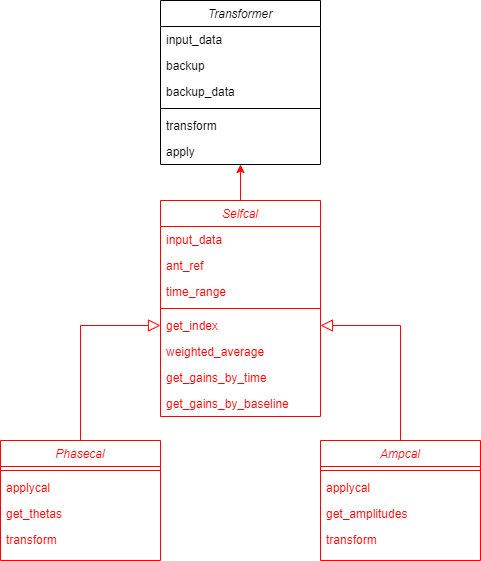
\includegraphics[scale=0.4]{images/Pyralysis-Self-calibration.png}
	\caption[Diagrama de clases Self-calibration]{Diagrama de clases Self-calibration. Fuente: Elaboración propia}
	\label{fig:selfcal_diagram}
\end{figure}

La clase \textit{Selfcal} está constituida por 3 atributos que son \texttt{input\_data} que representa el conjunto de datos, \texttt{ant\_ref} que es la antena de referencia y \texttt{time\_range} que es el rango de tiempo en el cual se quiere calibrar. Está además cuenta con los métodos siguientes: 

\begin{itemize}
    \item \texttt{get\_index}: Método que permite obtener los rangos de tiempos. Este se basa en el algoritmo \ref{alg:get_index}.
    \item \texttt{weighted\_average}: Realiza el promedio ponderado de los ángulos obtenidos.
    \item \texttt{get\_gains\_by\_time}: Realiza el agrupamiento mediante el rango de tiempo y el promedio ponderado para calcular los ángulos obtenidos. 
    \item \texttt{get\_gains\_by\_baseline}: Realiza el promedio ponderado de los ángulos agrupados por \textit{scan\_number}.
\end{itemize}

Las clases \textit{Phasecal} y \textit{Ampcal} tienen algunos métodos nombrados de igual manera pero realizan operaciones distintas. El método \texttt{applycal} permite aplicar los ángulos obtenidos a las visibilidades, donde en \textit{Phasecal} se aplica según la ecuación \ref{eq:applycal} y para \textit{Ampcal} se utiliza la ecuación \ref{eq:amp2}. Por otro lado, el método \texttt{get\_thetas} y \texttt{get\_amplitudes} aplican las ecuaciones \ref{eq:phase5} y \ref{eq:amp1} para así obtener los ángulos y las amplitudes respectivamente. 


\section{Bispectrum}

El método de \textit{Bispectrum} es creado en una clase del mismo nombre, la cual hereda de la clase \textit{Transformer} debido a que el objetivo de la clase \textit{Bispectrum} es realizar un reordenamiento del conjunto de datos ingresado. El diagrama de clases asociado a esta implementación es presentado en la Figura \ref{fig:bispectrum_diagram}.

\begin{figure}[!ht]
	\centering
	\captionsetup{justification=centering}
	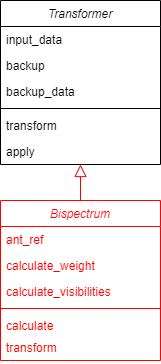
\includegraphics[scale=0.5]{images/Pyralysis-Bispectrum.png}
	\caption[Diagrama de clases para Bispectrum]{Diagrama de clases para Bispectrum. Fuente: Elaboración propia}
	\label{fig:bispectrum_diagram}
\end{figure}

Los atributos de la clase \textit{Bispectrum} son \texttt{ant\_ref} que es un número el cual indica la antena de referencia utilizada para filtrar las combinaciones iniciales, \texttt{calculate\_weight} y \texttt{calculate\_visibilities} son booleanos que indican si se debe calcular o no los pesos y visibilidades observadas en su formato \textit{Bispectrum}. El método \texttt{transform} reorganiza el conjunto de datos de tal manera de tener las visibilidades observadas, modelo y pesos en un arreglo con una dimensión igual a 3, de tal manera que cada dimensión de esta corresponde a una combinación de antenas ($ij$, $jk$ y $ki$). Por otro lado, el método \texttt{calculate} toma el conjunto de datos reordenado por \texttt{transform} y realiza la multiplicación de los datos para las combinaciones de antenas, sin embargo, para el calculo de los pesos se utiliza una variante de la ecuación \ref{eq:sigma} que esta dada por la ecuación \ref{eq:weight_bis} y para su obtención se debe tener en cuenta la ecuación \ref{eq:weights}.

\begin{equation}
    \label{eq:weights}
    w = \frac{1}{\sigma^2}
\end{equation}

\begin{equation}
    \label{eq:weight_bis}
    w_{bis} = \bigg( |V_{B}|^{2} \bigg[ \frac{1}{|V_{1}|^{2} w_{1}} + \frac{1}{|V_{2}|^{2} w_{2}} + \frac{1}{|V_{3}|^{2} w_{3}}\bigg] \bigg)^{-1}
\end{equation}

Para obtener una imagen con los datos obtenidos mediante la clase anterior es necesario definir la función y el gradiente para el \textit{Bispectrum} las cuales deben estar definidas en una clase, por lo mismo se tiene la clase \textit{Chi2Bis} que cumple con lo anterior. Esta clase cuenta con dos atributos llamados \texttt{model\_bispectrum} que es un tipo de objeto que se detallará mas adelante y \texttt{dataset} que es el conjunto de datos ingresado, además de contar con el método \texttt{function} que retorna el valor de la función objetivo definida en la ecuación \ref{eq:bispectrum_2} y el método \texttt{gradient} que retorna el valor del gradiente de la función objetivo y está definida por la ecuación \ref{eq:derivadaBis}.

\begin{figure}[!ht]
	\centering
	\captionsetup{justification=centering}
	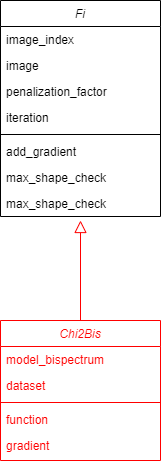
\includegraphics[scale=0.4]{images/Pyralysis-Bispectrum_Chi.png}
	\caption[Diagrama de clases para $\chi^2$ Bispectrum]{Diagrama de clases para $\chi^2$ Bispectrum. Fuente: Elaboración propia}
	\label{fig:bispectrumChi_diagram}
\end{figure}

Como se menciona anteriormente, la clase \textit{Chi2Bis} contiene un objeto llamado \texttt{model\_bispectrum} que viene de la clase del mismo nombre \textit{ModelBispectrum}. Este tiene el objetivo de calcular las visibilidades modelo \textit{Bispectrum} que posteriormente serán utilizadas en el cálculo de la función objetivo y su gradiente. En este \texttt{model\_bispectrum} es un método que permite el cálculo de las visibilidades modelo y su formato \textit{Bispectrum}. 

En el caso del optimizador para resolver la clase \textit{Chi2Bis} está dado por la clase \textit{NonLinearGradient} que hereda de la clase \textit{Optimizer}. Esta clase contiene 5 atributos que son \texttt{line\_search} que es el método de búsqueda lineal a utilizar para el paso del gradiente, \texttt{image} es la imagen inicial para el gradiente ($x_{0}$), \texttt{epsilon} es un número para evitar la división por cero, \textit{error} es el valor aceptable mínimo para el criterio de parada y \texttt{max\_iter} es la cantidad de iteraciones que realiza el gradiente. Para los métodos se tiene \texttt{run} que realiza la ejecución del gradiente conjugado y \texttt{polak\_rebiere} que aplica el método de Polak-Ribiere-Polyak para el calculo de $\beta$.

\begin{figure}[!ht]
	\centering
	\captionsetup{justification=centering}
	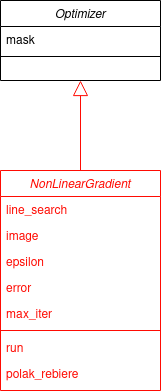
\includegraphics[scale=0.4]{images/Gradient.png}
	\caption[Diagrama de clases para Gradiente Conjugado]{Diagrama de clases para Gradiente Conjugado. Fuente: Elaboración propia}
	\label{fig:pyralysis_gradient}
\end{figure}

Un punto importante a destacar es que para la implementación de esta clase se utiliza el patrón de diseño \textit{Decorator} mencionado en la sección \ref{subsec:patrones}. Este se utiliza debido a la ventaja que trae al poder utilizar el método \texttt{transform} de la clase \textit{ModelVisibilities} y a la vez definir un método \texttt{transform} en \textit{ModelBispectrum} de manera que no se tenga que duplicar código y permitiendo respetar que el método \texttt{transform} en la clase \textit{Transformer} se define como un método abstracto, por lo que debe estar presente en todas sus clases hijas. 

\begin{figure}[!ht]
	\centering
	\captionsetup{justification=centering}
	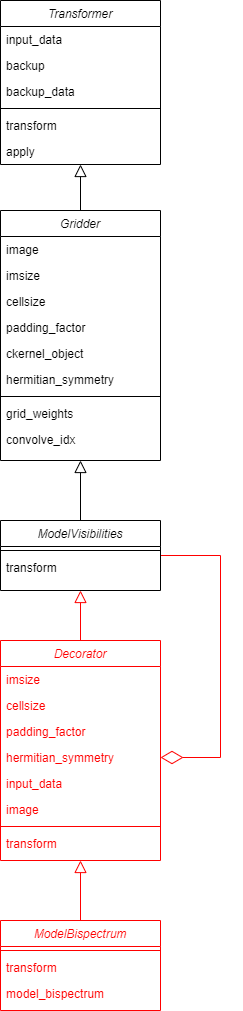
\includegraphics[scale=0.4]{images/Pyralysis-ModelBispectrum.png}
	\caption[Diagrama de clases para ModelBispectrum]{Diagrama de clases para ModelBispectrum. Fuente: Elaboración propia}
	\label{fig:modelBispectrum_diagram}
\end{figure}

Finalmente, para es necesaria la creación de una clase capaz de guardar los nuevos datos creados con \textit{Bispectrum}. La clase \textit{VisibilityBis} cumple con este objetivo al tener atributos que permiten el almacenamiento de las visibilidades y otros datos en su formato \textit{Bispectrum}, además esta clase hereda de la clase ya implementada en Pyralysis llamada \textit{VisibilitySet}, como se muestra en la Figura \ref{fig:visibilityBis_diagram}, de tal manera que se puede acceder a todos los atributos del conjunto de datos original. Los atributos que tiene la clase \textit{VisibilityBis} son los siguientes:

\begin{itemize}
    \item \texttt{antenna3}: Antena $k$ para combinación de antenas $i,j,k$.
    \item \texttt{bis\_data} y \texttt{bis\_model}: Visbilidades observadas y modelo respectivamente en su formato \textit{Bispectrum}.
    \item \texttt{bis\_uvw}: Datos UVW del conjunto de datos original ordenados en su formato \textit{Bispectrum}.
    \item \texttt{bis\_weight}: Pesos del conjunto de datos original ordenados en su formato \textit{Bispectrum}.
    \item \texttt{bis\_ant\_ref}: Antena de referencia utilizado para realizar el \textit{Bispectrum}.
\end{itemize}

\begin{figure}[!ht]
	\centering
	\captionsetup{justification=centering}
	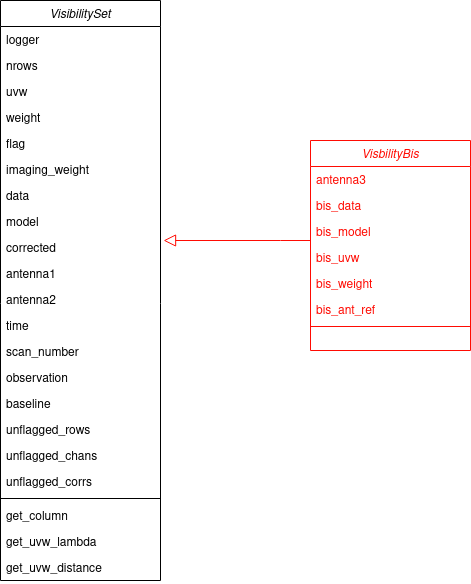
\includegraphics[scale=0.4]{images/Pyralysis-Visibility_bis.png}
	\caption[Diagrama de clases para VisibilityBis]{Diagrama de clases para VisibilityBis. Fuente: Elaboración propia}
	\label{fig:visibilityBis_diagram}
\end{figure}
